\documentclass[9pt, ngerman]{beamer}
\usetheme[progressbar=frametitle]{metropolis}
\usecolortheme[snowy]{owl}

\usepackage{babel}
\usepackage{csquotes}
\usepackage{booktabs}
\usepackage{siunitx}

\newcommand{\forward}[1]{\textbf{→ #1}}

\title{Der große Bierbrauworkshop}
\author{foo}

\begin{document}
\maketitle

% http://www.cloneabeer.com/CABebc.php
\definecolor{ebc4}{RGB}{255, 230, 153}
\definecolor{ebc8}{RGB}{255, 191, 66}
\definecolor{ebc12}{RGB}{248, 166, 0}
\definecolor{ebc20}{RGB}{222, 124, 0}
\definecolor{ebc35}{RGB}{134, 24, 0}
\definecolor{ebc61}{RGB}{90, 10, 2}
\definecolor{ebc79}{RGB}{54, 8, 10}

\begin{frame}{Vorstellung}
  \begin{itemize}
    \item Max \& Matze
    \item brauen seit etwa fünf Jahren
  \end{itemize}

  \begin{itemize}
    \item Mailingliste: \url{bier@lists.kit.edu}
    \item Brauergebnisse: \url{noerdbier.de}
    \item Technisches: \url{github.com/brewpeople}
  \end{itemize}
\end{frame}

\section{Einführung}

\begin{frame}{Definition}
  In Deutschland ist der Begriff und die Herstellung von \emph{Bier} durch die
  \emph{Verordnung zur Durchführung des Vorläufigen Biergesetzes} und das
  \emph{Vorläufige Biergesetz} von 1993 festgelegt.

  \begin{enumerate}
    \item[1.] Zur Bereitung von \textbf{untergärigem} Bier darf, abgesehen von den
      Vorschriften in den Absätzen 4 bis 6, nur \textbf{Gerstenmalz, Hopfen, Hefe und
      Wasser} verwendet werden.
    \item[2.] Die Bereitung von \textbf{obergärigem} Bier unterliegt derselben
      Vorschrift; es ist hierbei jedoch auch die Verwendung von \textbf{anderem
      Malz} und die Verwendung von technisch reinem Rohr-, Rüben- oder
      Invertzucker sowie von Stärkezucker und aus Zucker der bezeichneten Art
      hergestellten Farbmitteln zulässig.
  \end{enumerate}
\end{frame}
\begin{frame}{Definition}
  \begin{enumerate}
    \item[5.] An Stelle von Hopfen dürfen bei der Bierbereitung auch
      \textbf{Hopfenpulver} oder Hopfen in anderweit zerkleinerter Form oder
      Hopfenauszüge verwendet werden [\dots] Die Hopfenauszüge dürfen der
      Bierwürze nur \textbf{vor Beginn oder während der Dauer} des Würzekochens
      beigegeben werden.

    \item[6.] Als Klärmittel für Würze und Bier dürfen nur solche Stoffe
      verwendet werden, die mechanisch oder adsorbierend wirken und bis auf
      gesundheitlich, geruchlich und geschmacklich unbedenkliche, technisch
      unvermeidbare Anteile wieder ausgeschieden werden.
  \end{enumerate}
\end{frame}
\begin{frame}{Reinheitsgebot}
  \begin{itemize}
    \item Marketingbegriff aus dem 20. Jahrhundert mit Bezug auf eine
      bayerische Vorschrift von 1516
    \item In den 50ern und 60ern in Auseinandersetzungen um Zuckerzusätze
      in nicht-bayerischen später nicht-deutschen Bieren benutzt
    \item \emph{Tag des Deutschen Bieres} am 23. April erinnert an Erlassung
      einer neuen bayerischen Landesordnung im Jahr 1516, in der es unter
      anderem heißt:

      \enquote{\emph{Wir wöllen auch sonnderlichen / das füran
      allenthalben in unsern Stetten / Märckthen / unnd auf dem Lannde / zu
      kainem Pier / merer Stuckh / dann \textbf{allain Gersten / Hopffen / und
      Wasser} /
      genomen unnd gepraucht sölle werden.}}
  \end{itemize}
\end{frame}
\begin{frame}{Geschichtlicher Ursprung}
  Irgendwas mit Ägypten
\end{frame}
\begin{frame}{Das Tagesrezept}
  \begin{itemize}
    \item Pale Ale
  \end{itemize}
\end{frame}
\begin{frame}{Zutaten}
  \begin{itemize}
    \item Getreidemalze
    \item Wasser
    \item Hopfen
    \item Hefe
  \end{itemize}
\end{frame}
\begin{frame}{Malz}
  Die Stärke im Malz ist der Ausgangsstoff für den \forward{Zucker} der am Ende
  zu Kohlendioxid und Ethanol vergoren wird. Typische Malzgetreide sind
  \emph{Gerste} und \emph{Weizen}, weit seltener werden \emph{Roggen} und
  \emph{Dinkel} benutzt.

  Die \forward{Bierfarbe} hängt maßgeblich von der Farbe des Malzes ab, die
  durch Trocknungstemperatur beim \forward{Mälzen} festgelegt werden kann.
\end{frame}
\begin{frame}{Wasser}
\end{frame}
\begin{frame}{Hopfen}
  Der Hopfen fördert die \emph{Haltbarkeit} und bestimmt die
  \forward{Bitterkeit} eines Bieres.
\end{frame}
\begin{frame}{Hefe}
  Die Hefe führt zur \forward{Vergärung} des Zuckers zu Kohlendioxid und
  Ethanol.

  Alle Hefesorten lassen sich grob in \emph{untergärig} und \emph{obergärige}
  Hefen einteilen.  Untergärige Hefen benötigen Temperaturen zwischen \SIrange{4
  }{9}{\celsius}, während obergärige Hefen bereits bei Zimmertemperatur zur
  Gärung führen.
\end{frame}
\begin{frame}{Kennzahlen und -einheiten}
  \begin{block}{Bier}
    \begin{description}
      \item[IBU] International Bitter Units --- Bitterkeit
      \item[EBC] European Brewing Convention --- Bierfarbe
      \item[\textdegree P] Stammwürze \textdegree Plato
    \end{description}
  \end{block}

  \begin{block}{Hopfen}
    \begin{description}
      \item[\textalpha-Säure]  foo
    \end{description}
  \end{block}
\end{frame}
\begin{frame}{Bierfarbe}
  \tikzset{
    ebc bar/.style={
      rectangle,
      minimum width=2cm,
    }
  }
  \begin{table}
    \begin{tabular}{llll}
      \textbf{EBC} & \textbf{englisch} & \textbf{deutsch} & \textbf{Farbe}\\
      \midrule
      4--8  & pale & hell & \tikz {\node[ebc bar, left color=ebc4, right color=ebc8] {}} \\
      8--12 & golden, pale & gold & \tikz {\node[ebc bar, left color=ebc8, right color=ebc12] {}} \\
      12--20 & amber & bernstein & \tikz {\node[ebc bar, left color=ebc12, right color=ebc20] {}} \\
      20--35 & light brown, copper & kupfer & \tikz {\node[ebc bar, left color=ebc20, right color=ebc35] {}} \\
      35--60 & brown & braun & \tikz {\node[ebc bar, left color=ebc35, right color=ebc61] {}} \\
      60+ & dark brown, black & schwarz & \tikz {\node[ebc bar, left color=ebc61, right color=ebc79] {}}
    \end{tabular}
  \end{table}
\end{frame}
\begin{frame}{Untergärige Biertypen}
  \begin{table}
    \begin{tabular}{llllll}
      \textbf{Kategorie} & \textbf{StW \textdegree P} & \textbf{IBU} & \textbf{EBC} & \textbf{\% vol} \\
      \midrule
      Leichtes Lager & 7,0--13,8 & 8--30 & 4--12 & 2,8--6,0 \\
      Pils & 11,0--14,7 & 25--45 & 4--12 & 4,4--6,0 \\
      Europ. bernsteinf. Lager & 11,4--14,0 & 18--30 & 14--32 & 2,6--5,7 \\
      Dunkles Lager & 11,0--13,8 & 8--32 & 28--59 & 4,2--6,0 \\
      Bock & 15,7--28,0 & 16--35 & 12--59 & 6,3--14,0 \\
    \end{tabular}
  \end{table}
\end{frame}
\begin{frame}{Obergärige Biertypen -- Ales}
  \begin{table}
    \begin{tabular}{llllll}
      \textbf{Kategorie} & \textbf{StW \textdegree P} & \textbf{IBU} & \textbf{EBC} & \textbf{\% vol} \\
      \midrule
      English Pale Ale & 8,0--14,7 & 23--50 & 8--35 & 3,2--6,2 \\
      Scot./Irish Pale Ale & 7,6--30,1 & 10--35 & 18--49 & 2,5--10,0 \\
      American Ale & 11,2--14,7 & 20--45 & 10--69 & 4,3--6,2 \\
      English Brown Ale & 7,6--12,9 & 10--30 & 24--69 & 2,8--5,4 \\
      India Pale Ale & 12,4--21,6 & 40--120 & 12--30 & 5,0--10,0 \\
      Belg./Franz. Ale & 11,0--19,3 & 10--35 & 4--37 & 4,5--8,5 \\
      Belg. Starkbier & 15,2--25,9 & 15--40 & 6--43 & 6,0--11,0 \\
      Strong Ale & 14,7--28,0 & 30--120 & 16--43 & 6,0--12,0
    \end{tabular}
  \end{table}
\end{frame}
\begin{frame}{Obergärige Biertypen -- andere}
  \begin{table}
    \begin{tabular}{llllll}
      \textbf{Kategorie} & \textbf{StW \textdegree P} & \textbf{IBU} & \textbf{EBC} & \textbf{\% vol} \\
      \midrule
      Helles Hybrid & 9,5--13,6 & 15--30 & 5--12 & 2,1--5,6 \\
      Bernsteinf. Hybrid & 11,4--13,3 & 25--50 & 20--33 & 4,5--5,5 \\
      Porter & 10,0--21,6 & 18--50 & 33--69 & 4,5--9,5 \\
      Stout & 9,0--27,0 & 25--90 & 43--79 & 4,0--12,0 \\
      Weizen- u. Roggenbier & 11,0--21,6 & 8--30 & 4--49 & 4,3--8,0 \\
      Sauerbier & 7,1--18,0 & 0--25 & 4--43 & 2,8--8,0
    \end{tabular}
  \end{table}
\end{frame}

\section{Brauen}

\begin{frame}{Der Brauprozess im Überblick}
  \begin{enumerate}
    \item Mälzen und Schroten
    \item Einmaischen und Rasten \enquote{fahren}
    \item Läutern
    \item Hopfen kochen und Würzeklärung
    \item Vergärung und Lagerung
  \end{enumerate}
\end{frame}
{
\usebackgroundtemplate{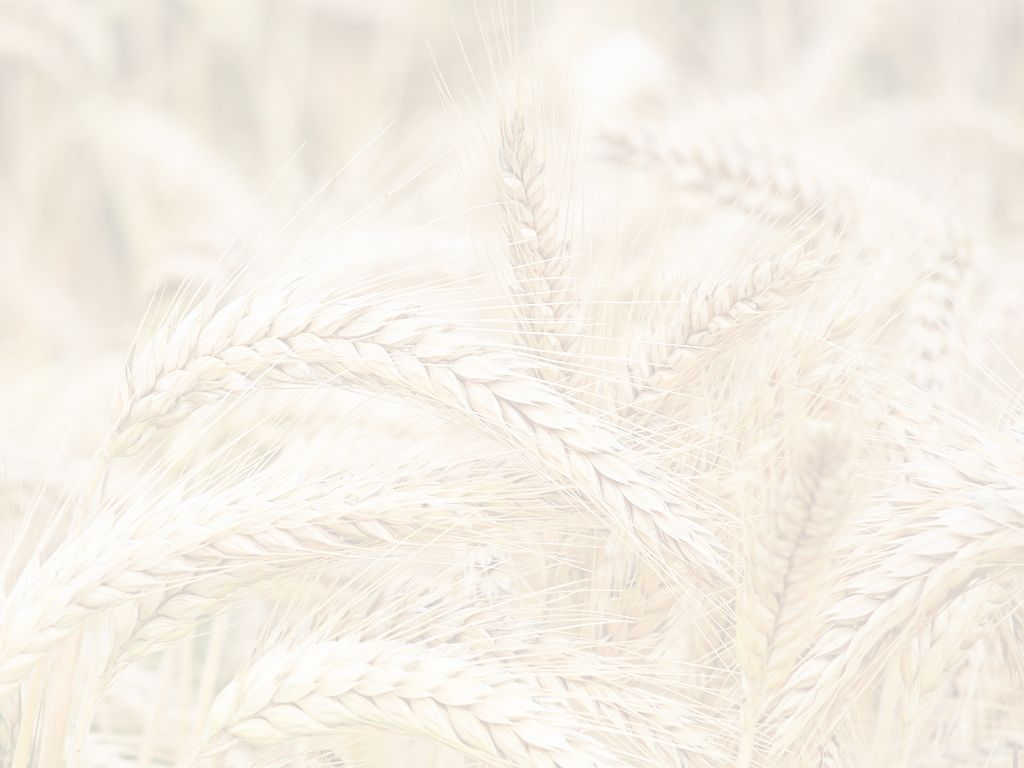
\includegraphics[width=\paperwidth]{cc0/gerste-pexels-photo-326082}}
\begin{frame}{Mälzen von Getreide}
  \begin{enumerate}
    \item \emph{Einweichen} der Gerste, Wassergehalt steigt von 12\% auf 42\%
    \item \emph{Keimung} und Abbau von Stärke und Eiweiß in Zucker und Aminosäuren
    \item Ende der Umsetzung durch \emph{Darren} (Trocknung) des Keims
    \item \emph{Schroten} statt vollständiges Mahlen erhält Spelze
  \end{enumerate}
\end{frame}
}
\begin{frame}{Maischen}
  \begin{enumerate}
    \item Aufweichen des Malzes bei \emph{Einmaischtemperatur}
    \item Umwandlung der Stärke bei verschiedenen \emph{Rasttemperaturen}
  \end{enumerate}
\end{frame}
\begin{frame}{Läutern}
  \begin{enumerate}
    \item Trennung des Korns und Eiweißes von der \emph{Würze}
  \end{enumerate}
\end{frame}
\begin{frame}{Hopfen}
  \begin{enumerate}
    \item Erhitzen der Würze bis auf Kochtemperatur
    \item Zugabe des \emph{Bitterhopfens}
    \item Zugabe des \emph{Aromahopfens} zum Ende
    \item Trennung der Würze vom Hopfen (z.B. mit \emph{Whirlpool})
  \end{enumerate}
  \begin{block}{Warum?}
    \begin{itemize}
      \item Aroma
      \item Haltbarkeit
    \end{itemize}
  \end{block}
\end{frame}
\begin{frame}{Minimalausstattung}
  \begin{itemize}
    \item Gefäß zum Kochen
    \item Läuterbottich mit Läuterblech
    \item Gärfass
  \end{itemize}
\end{frame}

% \begin{frame}{Sauberkeit}
%   Nach dem Hopfenkochen peinlichst drauf achten, die Würze nicht zu infizieren.
% \end{frame}

\end{document}
